% Generated by Sphinx.
\def\sphinxdocclass{report}
\documentclass[letterpaper,10pt,english]{sphinxmanual}
\usepackage[utf8]{inputenc}
\DeclareUnicodeCharacter{00A0}{\nobreakspace}
\usepackage{cmap}
\usepackage[T1]{fontenc}
\usepackage{babel}
\usepackage{times}
\usepackage[Bjarne]{fncychap}
\usepackage{longtable}
\usepackage{sphinx}
\usepackage{multirow}


\title{Tech Guide}
\date{December 19, 2013}
\release{13.11 Alpha}
\author{Chelsea School}
\newcommand{\sphinxlogo}{}
\renewcommand{\releasename}{Release}
\makeindex

\makeatletter
\def\PYG@reset{\let\PYG@it=\relax \let\PYG@bf=\relax%
    \let\PYG@ul=\relax \let\PYG@tc=\relax%
    \let\PYG@bc=\relax \let\PYG@ff=\relax}
\def\PYG@tok#1{\csname PYG@tok@#1\endcsname}
\def\PYG@toks#1+{\ifx\relax#1\empty\else%
    \PYG@tok{#1}\expandafter\PYG@toks\fi}
\def\PYG@do#1{\PYG@bc{\PYG@tc{\PYG@ul{%
    \PYG@it{\PYG@bf{\PYG@ff{#1}}}}}}}
\def\PYG#1#2{\PYG@reset\PYG@toks#1+\relax+\PYG@do{#2}}

\expandafter\def\csname PYG@tok@gd\endcsname{\def\PYG@tc##1{\textcolor[rgb]{0.63,0.00,0.00}{##1}}}
\expandafter\def\csname PYG@tok@gu\endcsname{\let\PYG@bf=\textbf\def\PYG@tc##1{\textcolor[rgb]{0.50,0.00,0.50}{##1}}}
\expandafter\def\csname PYG@tok@gt\endcsname{\def\PYG@tc##1{\textcolor[rgb]{0.00,0.27,0.87}{##1}}}
\expandafter\def\csname PYG@tok@gs\endcsname{\let\PYG@bf=\textbf}
\expandafter\def\csname PYG@tok@gr\endcsname{\def\PYG@tc##1{\textcolor[rgb]{1.00,0.00,0.00}{##1}}}
\expandafter\def\csname PYG@tok@cm\endcsname{\let\PYG@it=\textit\def\PYG@tc##1{\textcolor[rgb]{0.25,0.50,0.56}{##1}}}
\expandafter\def\csname PYG@tok@vg\endcsname{\def\PYG@tc##1{\textcolor[rgb]{0.73,0.38,0.84}{##1}}}
\expandafter\def\csname PYG@tok@m\endcsname{\def\PYG@tc##1{\textcolor[rgb]{0.13,0.50,0.31}{##1}}}
\expandafter\def\csname PYG@tok@mh\endcsname{\def\PYG@tc##1{\textcolor[rgb]{0.13,0.50,0.31}{##1}}}
\expandafter\def\csname PYG@tok@cs\endcsname{\def\PYG@tc##1{\textcolor[rgb]{0.25,0.50,0.56}{##1}}\def\PYG@bc##1{\setlength{\fboxsep}{0pt}\colorbox[rgb]{1.00,0.94,0.94}{\strut ##1}}}
\expandafter\def\csname PYG@tok@ge\endcsname{\let\PYG@it=\textit}
\expandafter\def\csname PYG@tok@vc\endcsname{\def\PYG@tc##1{\textcolor[rgb]{0.73,0.38,0.84}{##1}}}
\expandafter\def\csname PYG@tok@il\endcsname{\def\PYG@tc##1{\textcolor[rgb]{0.13,0.50,0.31}{##1}}}
\expandafter\def\csname PYG@tok@go\endcsname{\def\PYG@tc##1{\textcolor[rgb]{0.20,0.20,0.20}{##1}}}
\expandafter\def\csname PYG@tok@cp\endcsname{\def\PYG@tc##1{\textcolor[rgb]{0.00,0.44,0.13}{##1}}}
\expandafter\def\csname PYG@tok@gi\endcsname{\def\PYG@tc##1{\textcolor[rgb]{0.00,0.63,0.00}{##1}}}
\expandafter\def\csname PYG@tok@gh\endcsname{\let\PYG@bf=\textbf\def\PYG@tc##1{\textcolor[rgb]{0.00,0.00,0.50}{##1}}}
\expandafter\def\csname PYG@tok@ni\endcsname{\let\PYG@bf=\textbf\def\PYG@tc##1{\textcolor[rgb]{0.84,0.33,0.22}{##1}}}
\expandafter\def\csname PYG@tok@nl\endcsname{\let\PYG@bf=\textbf\def\PYG@tc##1{\textcolor[rgb]{0.00,0.13,0.44}{##1}}}
\expandafter\def\csname PYG@tok@nn\endcsname{\let\PYG@bf=\textbf\def\PYG@tc##1{\textcolor[rgb]{0.05,0.52,0.71}{##1}}}
\expandafter\def\csname PYG@tok@no\endcsname{\def\PYG@tc##1{\textcolor[rgb]{0.38,0.68,0.84}{##1}}}
\expandafter\def\csname PYG@tok@na\endcsname{\def\PYG@tc##1{\textcolor[rgb]{0.25,0.44,0.63}{##1}}}
\expandafter\def\csname PYG@tok@nb\endcsname{\def\PYG@tc##1{\textcolor[rgb]{0.00,0.44,0.13}{##1}}}
\expandafter\def\csname PYG@tok@nc\endcsname{\let\PYG@bf=\textbf\def\PYG@tc##1{\textcolor[rgb]{0.05,0.52,0.71}{##1}}}
\expandafter\def\csname PYG@tok@nd\endcsname{\let\PYG@bf=\textbf\def\PYG@tc##1{\textcolor[rgb]{0.33,0.33,0.33}{##1}}}
\expandafter\def\csname PYG@tok@ne\endcsname{\def\PYG@tc##1{\textcolor[rgb]{0.00,0.44,0.13}{##1}}}
\expandafter\def\csname PYG@tok@nf\endcsname{\def\PYG@tc##1{\textcolor[rgb]{0.02,0.16,0.49}{##1}}}
\expandafter\def\csname PYG@tok@si\endcsname{\let\PYG@it=\textit\def\PYG@tc##1{\textcolor[rgb]{0.44,0.63,0.82}{##1}}}
\expandafter\def\csname PYG@tok@s2\endcsname{\def\PYG@tc##1{\textcolor[rgb]{0.25,0.44,0.63}{##1}}}
\expandafter\def\csname PYG@tok@vi\endcsname{\def\PYG@tc##1{\textcolor[rgb]{0.73,0.38,0.84}{##1}}}
\expandafter\def\csname PYG@tok@nt\endcsname{\let\PYG@bf=\textbf\def\PYG@tc##1{\textcolor[rgb]{0.02,0.16,0.45}{##1}}}
\expandafter\def\csname PYG@tok@nv\endcsname{\def\PYG@tc##1{\textcolor[rgb]{0.73,0.38,0.84}{##1}}}
\expandafter\def\csname PYG@tok@s1\endcsname{\def\PYG@tc##1{\textcolor[rgb]{0.25,0.44,0.63}{##1}}}
\expandafter\def\csname PYG@tok@gp\endcsname{\let\PYG@bf=\textbf\def\PYG@tc##1{\textcolor[rgb]{0.78,0.36,0.04}{##1}}}
\expandafter\def\csname PYG@tok@sh\endcsname{\def\PYG@tc##1{\textcolor[rgb]{0.25,0.44,0.63}{##1}}}
\expandafter\def\csname PYG@tok@ow\endcsname{\let\PYG@bf=\textbf\def\PYG@tc##1{\textcolor[rgb]{0.00,0.44,0.13}{##1}}}
\expandafter\def\csname PYG@tok@sx\endcsname{\def\PYG@tc##1{\textcolor[rgb]{0.78,0.36,0.04}{##1}}}
\expandafter\def\csname PYG@tok@bp\endcsname{\def\PYG@tc##1{\textcolor[rgb]{0.00,0.44,0.13}{##1}}}
\expandafter\def\csname PYG@tok@c1\endcsname{\let\PYG@it=\textit\def\PYG@tc##1{\textcolor[rgb]{0.25,0.50,0.56}{##1}}}
\expandafter\def\csname PYG@tok@kc\endcsname{\let\PYG@bf=\textbf\def\PYG@tc##1{\textcolor[rgb]{0.00,0.44,0.13}{##1}}}
\expandafter\def\csname PYG@tok@c\endcsname{\let\PYG@it=\textit\def\PYG@tc##1{\textcolor[rgb]{0.25,0.50,0.56}{##1}}}
\expandafter\def\csname PYG@tok@mf\endcsname{\def\PYG@tc##1{\textcolor[rgb]{0.13,0.50,0.31}{##1}}}
\expandafter\def\csname PYG@tok@err\endcsname{\def\PYG@bc##1{\setlength{\fboxsep}{0pt}\fcolorbox[rgb]{1.00,0.00,0.00}{1,1,1}{\strut ##1}}}
\expandafter\def\csname PYG@tok@kd\endcsname{\let\PYG@bf=\textbf\def\PYG@tc##1{\textcolor[rgb]{0.00,0.44,0.13}{##1}}}
\expandafter\def\csname PYG@tok@ss\endcsname{\def\PYG@tc##1{\textcolor[rgb]{0.32,0.47,0.09}{##1}}}
\expandafter\def\csname PYG@tok@sr\endcsname{\def\PYG@tc##1{\textcolor[rgb]{0.14,0.33,0.53}{##1}}}
\expandafter\def\csname PYG@tok@mo\endcsname{\def\PYG@tc##1{\textcolor[rgb]{0.13,0.50,0.31}{##1}}}
\expandafter\def\csname PYG@tok@mi\endcsname{\def\PYG@tc##1{\textcolor[rgb]{0.13,0.50,0.31}{##1}}}
\expandafter\def\csname PYG@tok@kn\endcsname{\let\PYG@bf=\textbf\def\PYG@tc##1{\textcolor[rgb]{0.00,0.44,0.13}{##1}}}
\expandafter\def\csname PYG@tok@o\endcsname{\def\PYG@tc##1{\textcolor[rgb]{0.40,0.40,0.40}{##1}}}
\expandafter\def\csname PYG@tok@kr\endcsname{\let\PYG@bf=\textbf\def\PYG@tc##1{\textcolor[rgb]{0.00,0.44,0.13}{##1}}}
\expandafter\def\csname PYG@tok@s\endcsname{\def\PYG@tc##1{\textcolor[rgb]{0.25,0.44,0.63}{##1}}}
\expandafter\def\csname PYG@tok@kp\endcsname{\def\PYG@tc##1{\textcolor[rgb]{0.00,0.44,0.13}{##1}}}
\expandafter\def\csname PYG@tok@w\endcsname{\def\PYG@tc##1{\textcolor[rgb]{0.73,0.73,0.73}{##1}}}
\expandafter\def\csname PYG@tok@kt\endcsname{\def\PYG@tc##1{\textcolor[rgb]{0.56,0.13,0.00}{##1}}}
\expandafter\def\csname PYG@tok@sc\endcsname{\def\PYG@tc##1{\textcolor[rgb]{0.25,0.44,0.63}{##1}}}
\expandafter\def\csname PYG@tok@sb\endcsname{\def\PYG@tc##1{\textcolor[rgb]{0.25,0.44,0.63}{##1}}}
\expandafter\def\csname PYG@tok@k\endcsname{\let\PYG@bf=\textbf\def\PYG@tc##1{\textcolor[rgb]{0.00,0.44,0.13}{##1}}}
\expandafter\def\csname PYG@tok@se\endcsname{\let\PYG@bf=\textbf\def\PYG@tc##1{\textcolor[rgb]{0.25,0.44,0.63}{##1}}}
\expandafter\def\csname PYG@tok@sd\endcsname{\let\PYG@it=\textit\def\PYG@tc##1{\textcolor[rgb]{0.25,0.44,0.63}{##1}}}

\def\PYGZbs{\char`\\}
\def\PYGZus{\char`\_}
\def\PYGZob{\char`\{}
\def\PYGZcb{\char`\}}
\def\PYGZca{\char`\^}
\def\PYGZam{\char`\&}
\def\PYGZlt{\char`\<}
\def\PYGZgt{\char`\>}
\def\PYGZsh{\char`\#}
\def\PYGZpc{\char`\%}
\def\PYGZdl{\char`\$}
\def\PYGZhy{\char`\-}
\def\PYGZsq{\char`\'}
\def\PYGZdq{\char`\"}
\def\PYGZti{\char`\~}
% for compatibility with earlier versions
\def\PYGZat{@}
\def\PYGZlb{[}
\def\PYGZrb{]}
\makeatother

\begin{document}

\maketitle
\tableofcontents
\phantomsection\label{Index::doc}



\chapter{Moodle}
\label{moodle::doc}\label{moodle:tech-guide}\label{moodle:moodle}

\section{What is a Moodle?}
\label{moodle:what-is-a-moodle}
\href{https://moodle.org/about/}{Moodle} is a ``learning management system,'' a phrase used to refer to a class of software  ``for the administration, documentation, tracking, reporting and delivery of e-learning education courses or training programs.'' \footnote{
Ellis, Ryann K. (2009), Field Guide to Learning Management Systems, ASTD Learning Circuits.
}

Institutions rely on Moodle to fulfill different functions. At \href{http://chelseaschool.edu}{Chelsea School}, we rely on Moodle to augment on-campus courses or to provide hybrid courses.

Moodle is accessible via the Web at the following address: \href{http://chelseapride.org}{http://chelseapride.org} - note the address does not begin with \emph{www}.

Chelsea School's Moodle works best with Google Chrome, Mozilla Firefox, Opera, and Safari.


\section{Front Page (Main Conent Area)}
\label{moodle:front-page-main-conent-area}
We've made a significant effort to make Moodle's front page more accessible to more students.

In the past, students have been faced with a wall of text listing courses and course catalogs. Beginning this year, the main part of the Front Page begins with a more visual experience; the verbal components are still on the front page, but are now subordinate to the icon-driven experience.

Icons appear in three groups: Quicklinks for students, quicklinks for parents and guardians, and finally course categories.


\subsection{Links for Students}
\label{moodle:links-for-students}
In addition to a quicklink to course icons, students will find links for accessing other resources, such as their school E-mail accounts, Khan Academy, etc.

{\hfill\scalebox{1.000000}{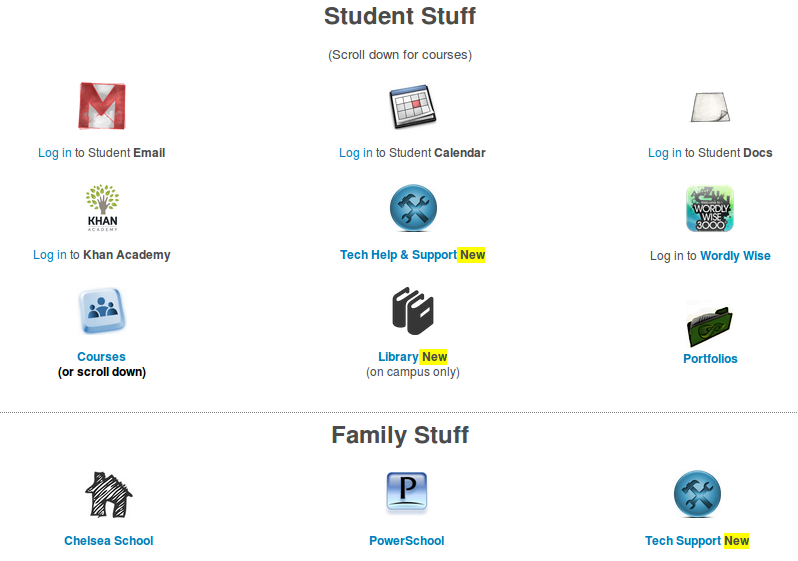
\includegraphics{moodle_student_stuff.png}}\hfill}


\subsection{Links for Parents and Guardians}
\label{moodle:links-for-parents-and-guardians}
This section includes links to PowerSchool, the student handbook, etc.

{\hfill\scalebox{1.000000}{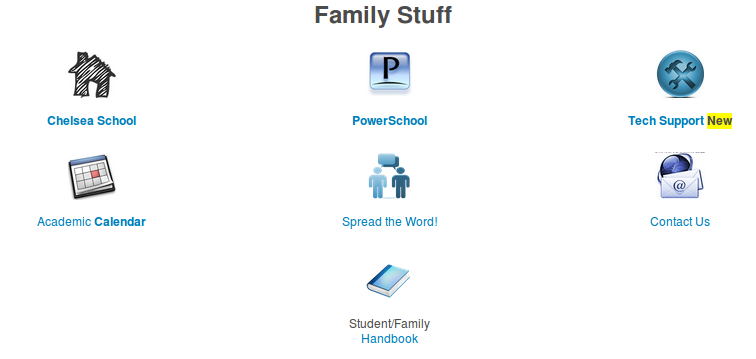
\includegraphics{family_stuff.png}}\hfill}


\subsection{Academic Departments}
\label{moodle:academic-departments}
We've limited the amount of text the user has to cut through by linking directly to course departments: Science, Technology, English/Language Arts, etc.

{\hfill\scalebox{1.000000}{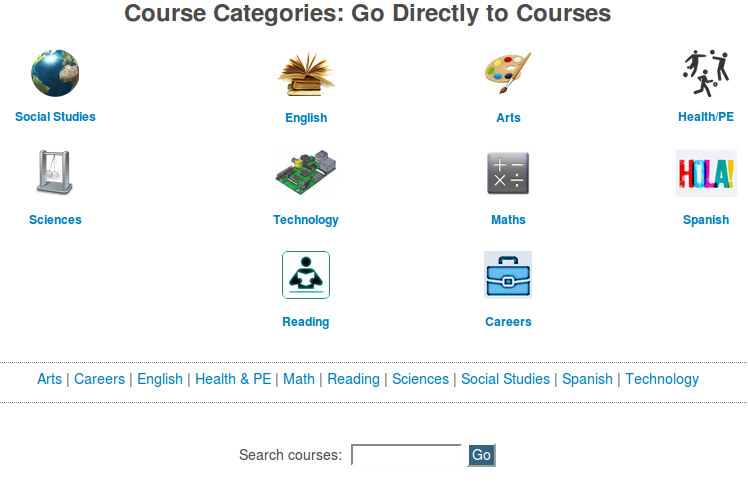
\includegraphics{course_icons.png}}\hfill}


\subsection{Courses by Category}
\label{moodle:courses-by-category}
Wall of text. More direct path to courses, but not the best way to serve many in our community.

{\hfill\scalebox{1.000000}{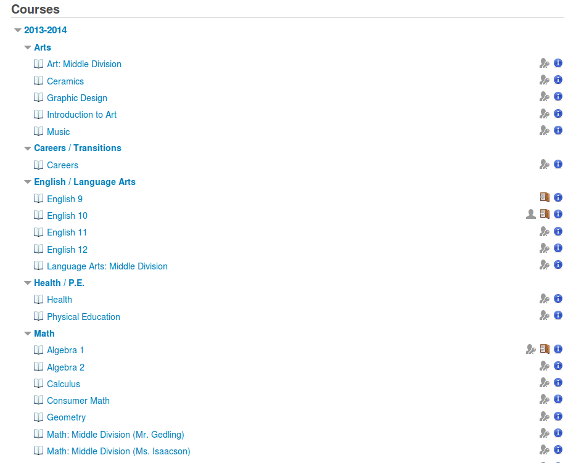
\includegraphics{moodle_text.png}}\hfill}


\section{Front Page (Left Sidebar)}
\label{moodle:front-page-left-sidebar}

\subsection{Logging In (Students Only)}
\label{moodle:logging-in-students-only}
To the immediate left of the front page content area is a sidebar for navigation. It is divided into blocks. The top block is for logging in to Moodle.

Logging in requires a username and complex password. Both are provided by a student's advisor and cannot be changed by the student. The pattern for student usernames is \textless{}lastname\textgreater{}\textless{}first initial\textgreater{} (all lower case). To log in, enter the username in the username field and the password into the password field; press enter or click \emph{Login} to submit credentials.

{\hfill\scalebox{1.000000}{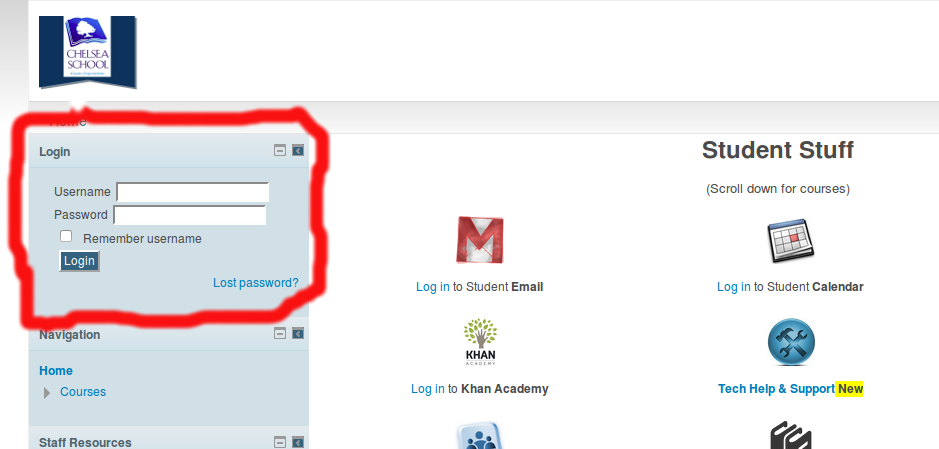
\includegraphics{login_block.png}}\hfill}

After a brief wait, successful login will be indicated at the top right of the page, which should indicate that the student is the logged in user.

Forgotten passwords can be recovered by advisors and their colleagues. However, students who get stuck logging in to Moodle from home can contact \href{http://chelseapride.org/helpdesk}{helpdesk} at \href{http://chelseapride.org/helpdesk}{http://chelseapride.org/helpdesk}.

There are icons for helpdesk in both the Student's section of the front page and the Parents' and Guardians' section of the front page.


\section{Parent \& Guardian Access}
\label{moodle:parent-guardian-access}
Parents and guardians are discouraged from logging in to student accounts; we understand, however, that in some cases it can be helpful.

With that in mind, we've configured all available courses to be either:
\begin{enumerate}
\item {} 
Available to the public; or

\item {} 
Available with a passcode.

\end{enumerate}

At Chelsea School, restricted courses have been configured to provide guest access to guests with a course passcode.

The passcode with which parents and guardians can access all restricted courses is \_\_\_\_\_\_\_\_\_\_\_\_\_\_\_\_\_.

To access a course as a guest,
\begin{enumerate}
\item {} 
Navigate to the desired course;

\item {} 
Click on ``Login as Guest;''

\item {} 
Enter ``Guest Access Password'' and click ``Submit.''

\end{enumerate}


\section{Navigating to a Course}
\label{moodle:navigating-to-a-course}
Moodle provides several ways to access courses:
\begin{enumerate}
\item {} 
On the left sidebar of the front page, there's a ``block'' called ``Navigation.'' Select ``courses'' in the Navigation block to expand to show course categories; to view individual courses within a category, select the category; the contents will expand to show available courses with abbreviated names. Click on the name of the course to access it.

\item {} 
In the ``Student Stuff'' section of the front page (main content area), there's an icon labeled ``courses.'' Click on the icon to see icons for each department in the main content area of the front page. Click on the department of the desired course to reveal a list of the department's courses in the main content area. Browse for the name of the desired course and click on it.

\item {} 
From the front page, one can search for courses by scrolling down to below the course categories section in the main content area. To search for a course, accurately enter a portion of the course name and press enter (or click the blue ``Go'' button.

\item {} 
To browse the full course catalog by department, scroll down to just past the search field on the front page (main content area). Click on the desired course to access it.

\end{enumerate}


\section{Resources}
\label{moodle:helpdesk}\label{moodle:resources}\begin{itemize}
\item {} 
\href{http://youtu.be/PSwbhCqLSQI}{Introducing Parents to Moodle} (YouTube)

\item {} 
\href{http://docs.moodle.org/26/en/Moodle\_site\_-\_basic\_structure}{Moodle Site Structure} (Documentation)

\item {} 
\href{http://learning.oconeeschools.org/course/view.php?id=477}{Moode for Students and Parents} (Frequently Asked Questions)

\end{itemize}

\index{moodle}\index{LMS}\index{CMS}\index{courses}\index{departments}\index{key}\index{passcode}\index{password}\index{login}\index{logging in}\index{credentials}\index{icons}\index{visual}

\chapter{PowerSchool}
\label{powerschool::doc}\label{powerschool:powerschool}\label{powerschool:index-0}

\section{What is PowerSchool?}
\label{powerschool:what-is-powerschool}
Pearson's \href{http://chelseaschool.powerschool.com/}{PowerSchool} is a web-based shool information system. At its foundation, PowerSchool is used to record, report, and view student grades, attendance, and reports. It provides parents and guardians access through a Web browser via its ``Parent Portal.''


\section{Credentials}
\label{powerschool:credentials}
Credentials for \href{http://chelseaschool.powerschool.com/}{PowerSchool} Parent Portal were generated for each student's parents and guardians and sent via E-mail at the beginning of Quarter 1.

If you've misplaced your login credentials, please contact \href{http://chelseapride.org/helpdesk}{helpdesk}.


\section{Accessing PowerSchool}
\label{powerschool:accessing-powerschool}
It's been our experience that \href{http://chelseaschool.powerschool.com/}{Powerschool} is best accessed using Mozilla \href{http://www.mozilla.org/en-US/firefox/new/}{Firefox}. We have compelling evidence that Google Chrome is not compatible at this point.

Using \href{http://www.mozilla.org/en-US/firefox/new/}{Firefox}, navigate to \href{http://chelseaschool.powerschool.com/}{http://chelseaschool.powerschool.com/}.

Alternatively, navigate to \href{http://chelseapride.org}{Moodle} (\href{http://chelseapride.org}{http://chelseapride.org}) and click the \href{http://chelseaschool.powerschool.com/}{PowerSchool} icon on the front page under either ``Student Stuff'' or ``Family Stuff.''

You will prompted to enter credentials for \href{http://chelseaschool.powerschool.com/}{PowerSchool}. Enter the correct credentials, being mindful of capitalization, and click the ``Sign In'' button. (From this page, you may also follow links to recover a lost username or password.)

{\hfill\scalebox{1.000000}{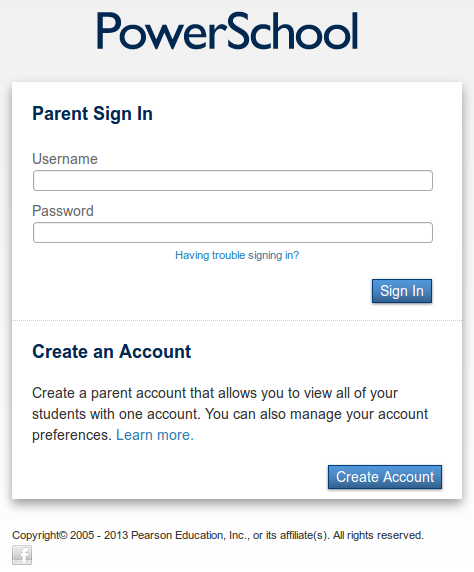
\includegraphics{pslogin.png}}\hfill}

If you have trouble accessing \href{http://chelseaschool.powerschool.com/}{PowerSchool} the first time, please contact \href{http://chelseapride.org/helpdesk}{helpdesk} via the Web. Please include the following information: your name, the student's name, and a description of the problem your having in as much detail as you can provide.


\section{Resources}
\label{powerschool:resources}\begin{itemize}
\item {} 
\href{http://youtu.be/SzF4wF4fglY}{PowerSchool Parent Portal} (YouTube)

\item {} 
\href{http://youtu.be/7z5rOk-89OE}{PowerSchool: Parent Portal Tutorial} (YouTube)

\item {} 
\href{http://youtu.be/YFS0n2D8ri4}{Viewing Child's Grades in PowerSchool Parent Portal} (YouTube)

\item {} 
Parent Portal User Guide (PDF)

\end{itemize}

\index{grades}\index{attendance}\index{transcripts}\index{reports}\index{students}\index{PowerSchool}\index{Pearson}\index{SIS}\index{parents}\index{guardians}\index{records}

\chapter{Lexia}
\label{lexia::doc}\label{lexia:index-0}\label{lexia:lexia}

\section{What is Lexia Reading?}
\label{lexia:what-is-lexia-reading}
Lexia provides explicit, systematic, personalized learning on foundational reading skills for students of all abilities, and delivers norm-referenced performance data and analysis without interrupting the flow of instruction to administer a test. This research-proven, technology-based approach accelerates reading skills development, predicts students’ year-end performance and provides teachers data-driven action plans to help differentiate instruction. \footnote{
\href{http://www.lexialearning.com/product}{http://www.lexialearning.com/product}
}

Lexia Strategies for Older Students is designed for remedial students in grades 6 and above, at a Tier II and Tier III level. The program focuses on foundational reading skills, starting at first grade skill levels, with a more mature, age-appropriate interface and a range of content. \footnote{
\href{http://www.lexialearning.com/product\#sos}{http://www.lexialearning.com/product\#sos}
}


\section{Credentials}
\label{lexia:credentials}
To use Lexia Reading at home, you'll need Chelsea School's \emph{Customer Code}. Obtain the code - with dashes; you may choose to record it below.

Customer Code: \_\_\_\_\_\_\_\_\_\_\_\_\_\_\_\_\_\_\_\_\_\_\_\_\_\_\_\_\_\_\_\_\_

Your student will have been provided a username and password. Consider recording them below:

Lexia Username: \_\_\_\_\_\_\_\_\_\_\_\_\_\_\_\_\_\_\_\_

Lexia Password: \_\_\_\_\_\_\_\_\_\_\_\_\_\_\_\_\_\_\_\_


\section{Installing Lexia Reading at Home}
\label{lexia:installing-lexia-reading-at-home}

\subsection{Download the Installer}
\label{lexia:download-the-installer}\begin{enumerate}
\item {} 
Use a browser to navigate to \href{http://www.lexialearning.com}{http://www.lexialearning.com}.

\item {} 
Click \emph{Downloads} in the upper-right hand corner.

\item {} 
Accept the license agreement.

\item {} 
Click the version of the software for your system to begin downloading.

\end{enumerate}


\subsection{Install and Configure Lexia Reading}
\label{lexia:install-and-configure-lexia-reading}

\subsubsection{Windows Users}
\label{lexia:windows-users}\begin{enumerate}
\item {} 
Double-click the Lexia Reading.exe installer file that you downloaded.

\item {} 
Follow the screen prompts until you see the Customer Code screen.

\item {} 
Type in the customer code you received from the school (include dashes).

\end{enumerate}


\subsubsection{Mac Users}
\label{lexia:mac-users}\begin{enumerate}
\item {} 
Double-click the Lexia volume that you downloaded. Drag and drop the Lexia icon from the left to the Applications folder on the right to install.

\item {} 
In the Applications folder, click the Lexia icon. The Settings screen displays.

\item {} 
Type in the customer code you received from the school (include dashes).

\end{enumerate}


\section{Resources}
\label{lexia:resources}
Lexia School to Home support: \href{http://www.lexialearning.com/lexiasupport/school-to-home}{http://www.lexialearning.com/lexiasupport/school-to-home}.

\index{reading}\index{lexia}\index{lexiareading}\index{literacy}\index{phonemic awareness}

\chapter{Kurzweil 3000}
\label{kurzweil::doc}\label{kurzweil:index-0}\label{kurzweil:kurzweil-3000}

\section{What is Kurzweil 3000}
\label{kurzweil:what-is-kurzweil-3000}
\href{http://www.kurzweiledu.com/products/kurzweil-3000-firefly-overview.html}{Kurzweil} 3000 provides a comprehensive suite of supports for struggling students, including reading, writing, study skills, and test taking.

{\hfill\scalebox{1.000000}{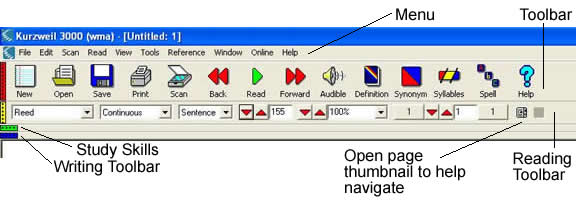
\includegraphics{KurzweilCrop.jpg}}\hfill}

At Chelsea School, many students are introduced to \href{http://www.kurzweiledu.com/products/kurzweil-3000-firefly-overview.html}{Kurzweil} 3000 as powerful tool for composition, editing, and revision.

\href{http://www.kurzweiledu.com/products/kurzweil-3000-firefly-overview.html}{Kurzweil} 3000 was pioneering in the areas of text to speech (\textbf{TTS}) and optical character recognition.

According to Kurzweil's promotional copy: Using natural sounding voices, \href{http://www.kurzweiledu.com/products/kurzweil-3000-firefly-overview.html}{Kurzweil} 3000 reads text aloud to students, allowing them to follow along as the text is highlighted and spoken at a self-adjusted pace. Additional literacy tools use a multisensory approach to engage students as they develop language fluency, comprehension and retention. As a result, students with language-based learning differences are able to read at a higher level than they could independently and achieve success alongside their peers.

{\hfill\scalebox{1.000000}{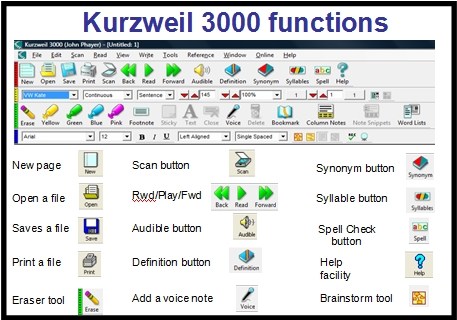
\includegraphics{jp-kurzweil-1.jpg}}\hfill}

Some students' IEPs provide for TTS accomodations during state testing. That accomodation is provided through \href{http://www.kurzweiledu.com/products/kurzweil-3000-firefly-overview.html}{Kurzweil} 3000 -- but only when the student is familiar with the software.


\subsection{Key Features}
\label{kurzweil:key-features}\begin{itemize}
\item {} 
Text-to-speech in seven languages

\item {} 
Reads any digital text aloud, including the Internet

\item {} 
Multiple reference sources, including bi-lingual

\item {} 
Translations to any Google supported language

\item {} 
Highlighters and sticky notes

\item {} 
Vocabulary study guides

\item {} 
Graphic organizer

\item {} 
Writing templates

\item {} 
Word prediction

\item {} 
Talking spell checker

\item {} 
Direct access to Bookshare and other online content providers \footnote{
Chelsea School has access to the Bookshare collection.
}

\end{itemize}


\subsection{In the Home}
\label{kurzweil:in-the-home}
Chelsea School has opted to use Web-based licensing for Kurzweil- 3000. This ``floating license'' permits students use \href{http://www.kurzweiledu.com/products/kurzweil-3000-firefly-overview.html}{Kurzweil} 3000 from a home PC with internet connectivity. \footnote{
With our Tech Mobile, Chelsea School staff are able to offer to install Kurzweil 3000 on a student's home PC.
}


\subsection{Resources}
\label{kurzweil:resources}\begin{itemize}
\item {} 
\href{http://www.kurzweiledu.com/products/kurzweil-3000-firefly-overview.html}{Kurzweil} 3000 Product Information: \href{http://www.kurzweiledu.com/products/kurzweil-3000-firefly-overview.html}{http://www.kurzweiledu.com/products/kurzweil-3000-firefly-overview.html}

\item {} 
\href{http://www.kurzweiledu.com/products/kurzweil-3000-firefly-overview.html}{Kurzweil} 3000 on YouTube (6:21): \href{http://youtu.be/KbuJFsqu6x4}{http://youtu.be/KbuJFsqu6x4}

\item {} 
Getting Started with \href{http://www.kurzweiledu.com/products/kurzweil-3000-firefly-overview.html}{Kurzweil} 3000 (PDF): \href{https://www.kurzweiledu.com/files/v13/Getting\_Started\_With\_Kurzweil\_3000\_WIN.pdf}{https://www.kurzweiledu.com/files/v13/Getting\_Started\_With\_Kurzweil\_3000\_WIN.pdf}

\end{itemize}

\index{tts}\index{TTS}\index{text to speech}\index{accessibility}\index{Kurzweil 3000}\index{IEP}\index{Kurzweil}\index{reading}\index{writing}\index{study skills}\index{literacy}

\chapter{Tech Support}
\label{helpdesk::doc}\label{helpdesk:tech-support}\label{helpdesk:index-0}\label{helpdesk:kurzweil}

\section{Helpdesk}
\label{helpdesk:helpdesk}
\href{http://chelseapride.org/helpdesk/}{Helpdesk} is available to users via the Web using an application called \href{http://chelseapride.org/helpdesk/}{OSTicket}.

To get help via the Web, browse to \href{http://chelseapride.org/helpdesk/}{http://chelseapride.org/helpdesk/}. When the page loads, you'll have an opportunity to \emph{Open a new ticket} (green button, middle-left side of the page.

To open a new ticket, you must provide your name, Email address, and a brief subject line - just as you would for an Email. For the help topic, you must select \emph{support} from the drop-down menu.

In the message field, please articulate your support needs in as much detail as possible, Explain the problem as well how to reproduce it, what you've tried to solve it, etc.

{\hfill\scalebox{1.000000}{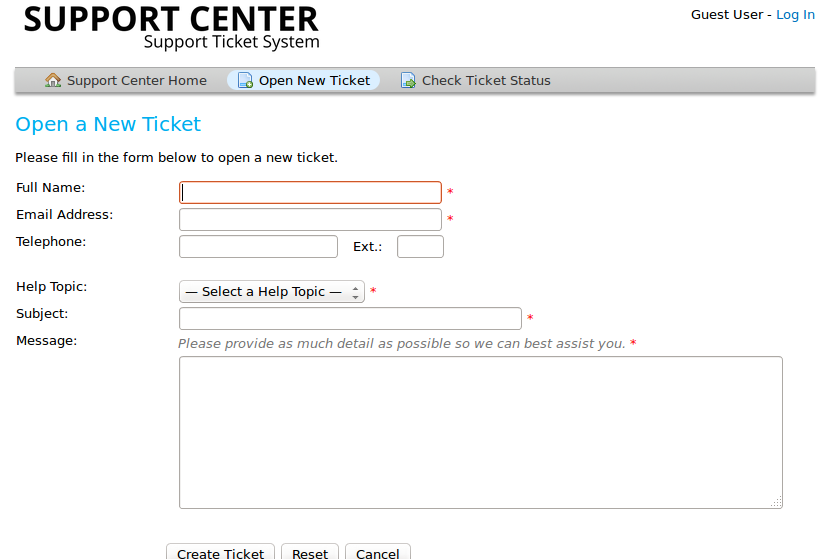
\includegraphics{osticket.png}}\hfill}

\textbf{Important}: Please include the name of your Chelsea School student in the \emph{message} field.


\section{Tech Mobile}
\label{helpdesk:tech-mobile}\label{helpdesk:osticket}
If you are having trouble installing Lexia at home or need Kurzweil installed, Chelsea School has a tech mobile program that, upon request, can come to your home.

If you would like to schedule an appointment with the tech mobile program, please contact Karen Gallo or Sabre Goldman.  The tech mobile program can also offer assistance with PowerSchool and Moodle.

\index{helpdesk}\index{tech support}\index{support}\index{troubleshooting}\index{OSticket}\index{tech mobile}

\chapter{Additional Technology Resources}
\label{resources::doc}\label{resources:index-0}\label{resources:additional-technology-resources}

\section{Text to Speech}
\label{resources:text-to-speech}

\subsection{TextAloud}
\label{resources:textaloud}\begin{itemize}
\item {} 
Free trial available

\item {} 
Purchase price is \$29.95

\item {} 
Integrates with premium voice packs from AT\&T and Nuance

\item {} 
Exports text to MP3

\item {} 
Product URL: \href{http://www.nextup.com/TextAloud/}{http://www.nextup.com/TextAloud/}

\end{itemize}


\subsection{ReadPlease 2003}
\label{resources:readplease-2003}
\href{https://sites.google.com/a/readerpal.com/readplease/}{ReadPlease} will read any text you see on your screen. This can be from your browser, email, word processor, spreadsheet, or any program which displays text.
\begin{itemize}
\item {} 
Was premium software, now unsupported and at end of life. Nevertheless, effective TTS software that the developers have been kind enough to offer offer a free registration code.

\item {} 
Registration Name: \textbf{READPLEASE}

\item {} 
Registration Code: \textbf{939718100231563}

\item {} 
Direct Download:  \href{https://sites.google.com/a/readerpal.com/readplease/home/SetupReadPlease2003.zip}{https://sites.google.com/a/readerpal.com/readplease/home/SetupReadPlease2003.zip}

\end{itemize}


\subsection{WriteType}
\label{resources:writetype}
WriteType is a free (and open source) program that helps students experience success in writing.  It is designed especially for schools to transform technology from a barrier into an opportunity for success.  Some major features include:
\begin{itemize}
\item {} 
Word Completion — As students type, word suggestions appear on the right-hand side of the screen to complete the word being typed.  Clicking on the desired word will finish the word.  WriteType will also learn a student’s habits over time and make more relevant suggestions based on what has already been written.

\item {} 
Reading Back the Document — WriteType will read back written text, allowing students to catch errors they may not have caught reading it back themselves. It will also, optionally, read back words as they are typed.

\item {} 
Highlighting — Sections of the document can be quickly highlighted while typing or while listening to the document being read back. This lets students quickly flag areas they need to go back and review.

\item {} 
Grammar checking — WriteType will underline simple grammar and formatting mistakes in the document, and offer to make the necessary revision.

\item {} 
Auto-correction — Common errors, such as typing isnt instead of isn’t, will be corrected automatically without the need for intervention.

\item {} 
Multi-lingual — WriteType is available in English, Spanish, Dutch, Italian, Russian, Bulgarian, and Basque.

\item {} 
Download WriteType for Windows: \href{http://writetype.bernsteinforpresident.com/download/}{http://writetype.bernsteinforpresident.com/download/}

\end{itemize}


\section{Speech to Text}
\label{resources:id2}\label{resources:speech-to-text}\begin{itemize}
\item {} 
Nuance \href{http://www.nuance.com/dragon/index.htm}{Dragon} Naturally Speaking
\begin{quote}

\href{http://www.nuance.com/dragon/index.htm}{Dragon} is best-selling speech recognition software. It turns your talk into text and can make virtually any computer task easier and faster. From capturing ideas and creating documents, to email and searching the web, to using simple voice commands to control many of the popular programs you use every day at home, work – and beyond.
Mobile apps for Dragon are available for Android and iOS devices. Students can dictate their writing assignments into their smart devices and then transfer their work to school computers.
\end{quote}

\end{itemize}


\section{Fonts}
\label{resources:fonts}\begin{itemize}
\item {} 
\href{http://opendyslexic.org/}{OpenDyslexic}
\begin{quote}

\href{http://opendyslexic.org/}{OpenDyslexic} is a new open sourced font created to increase readability for readers with dyslexia. The typeface includes regular, bold, italic, and bold-italic styles. It is being updated continually and improved based on input from dyslexic users. There are no restrictions on using OpenDyslexic outside of attribution.
\end{quote}

\item {} 
Lexia \href{http://www.k-type.com/?p=520}{Readable}
\begin{quote}

Lexia \href{http://www.k-type.com/?p=520}{Readable} was designed for maximum legibility, an attempt to capture the strength and clarity of Comic Sans without the comic book associations. Features like the non-symmetrical b and d, and the handwritten forms of a and g may help dyslexic readers.
In 2013, many more accented characters were added to each weight to complete the Latin Extended-A range. Some minor outline, spacing and kerning improvements were also made.
The Regular and Bold weights can be used freely without a licence by educational and charitable institutions as well as for personal use by individuals.
Licences for the Italic/BoldItalic and Heavy/Outline packages are available from K-Type.
\end{quote}

\item {} 
Tiresias \href{http://www.fontsquirrel.com/fonts/Tiresias-Infofont}{Infofont}
\begin{quote}

Designed by The Royal National Institute for the Blind
\end{quote}

\end{itemize}


\section{Browser Extensions}
\label{resources:browser-extensions}

\subsection{Google Chrome}
\label{resources:google-chrome}
TBA


\subsection{Mozilla Firefox}
\label{resources:mozilla-firefox}
TBA


\section{Mobile Apps}
\label{resources:mobile-apps}

\subsection{Homework and Agenda Apps}
\label{resources:homework-and-agenda-apps}\begin{itemize}
\item {} 
myHomework App - prioritize assignments, set up pop-up reminders, and syncs to all of your devices

\item {} 
Everstudent - color-code assignments and syncs with Evernote

\end{itemize}


\subsection{Portfolios}
\label{resources:portfolios}\begin{itemize}
\item {} 
Mahara - keep a digital portfolio and build customizeable resumes

\end{itemize}


\subsection{Text to Speech}
\label{resources:id3}\begin{itemize}
\item {} 
Voice-Dream - extract from mutiple file types and has a dyslexia-friendly font

\end{itemize}


\subsection{Study Skills and Writing Apps}
\label{resources:study-skills-and-writing-apps}\begin{itemize}
\item {} 
iThoughts - mindmapping app that helps with planning and organization and exports to PowerPoint or Word

\item {} 
Dictionary.com Flashcards - customizeable flashcards with pronunication and monitors progress

\item {} 
Dragon Dictation - speech-to-text app

\item {} 
Evernote - organizes and syncs notes

\end{itemize}
\begin{itemize}
\item {} 
\emph{genindex}

\item {} 
\emph{search}

\end{itemize}



\renewcommand{\indexname}{Index}
\printindex
\end{document}
